\chapter{Breast Cancer}\label{chap:breastcancer}

\section*{}

In this chapter, an overview of the breast anatomy and physiology is presented along side with concepts and treatments regarding breast cancer. The chapter focuses on some of the available types of surgery, and the factors that can influence the aesthetic outcome of those treatments. Not only the anatomical explanations, but also the impacts of breast cancer treatment on the patient's quality of life are described in the following.

\section{Breast Physiology} \label{sec:physiology}

The breast is made up of different layers, but predominantly by fat and glandular tissue, having as boundaries the second and the sixth ribs, vertically, and the lateral edge of the sternum and the mid axillary line, medially. Through a woman's aging, the breast suffers transformation during the puberty and menopause, where the ratio between the fat and glandular tissues may vary as well as the blood supply and the lymphatic drainage \cite{Ellis2013}.
On adulthood, the mammary gland has about 15 to 20 lobes that converge to the nipple through milk ducts. The milk ducts are surrounded by dense connective tissue, known as fibroglandular tissue or Cooper's ligaments. The majority of the breast, about two thirds, is placed over the pectoral muscle, while its shape is established and maintained by the skin and the Cooper's ligaments \cite{apenn,Vavourakis2016}. A breast's structure is represented in Figure \ref{fig:breast structure}.

\begin{figure}[H]
\begin{center}
	\leavevmode
    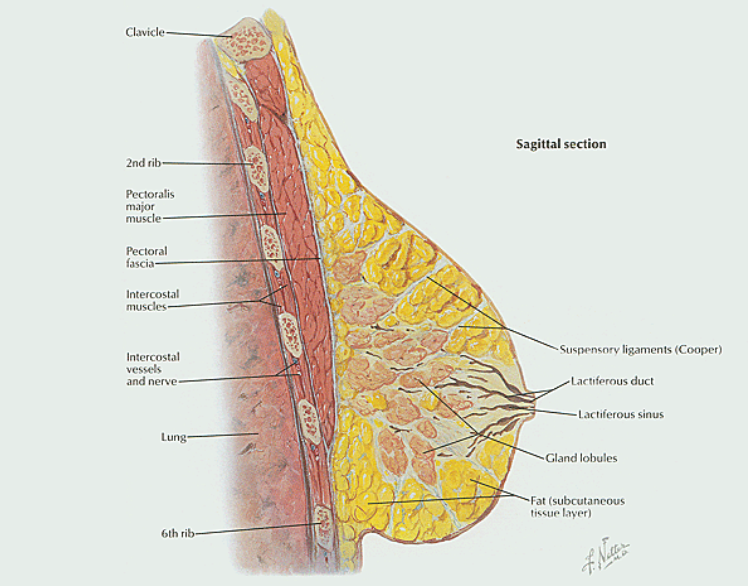
\includegraphics[width=0.8\textwidth]{breast_anat}
    \caption[Breast Structure]{Breast's Structure \cite{Witmer2004}}
    \label{fig:breast structure}
\end{center}
\end{figure}

\section{Breast Cancer and Incidence} \label{sec:incidence}

Breast cancer is caused by the presence of a malignant tumor, known as carcinoma, developed from the breast cells. Despite of being more common in women (99\%), this disease can also affect men (1\%). Portugal follows the same trend as developed countries regarding the diagnosed cases of breast cancer per years. \footnote{\url{http://www.who.int/cancer/country-profiles/prt_en.pdf?ua=1}}

The tumor, regarding its location, can be associated with one or more of the following 6 regions of the breast: upper-inner, upper-outer, lower-inner, lower-outer, nipple and areola complex or axillary tail. Usually the axillary tail is also considered as upper-outer region. Figure \ref{fig:breast regions} shows the breast regions division into quadrants and the nipple and areola complex.

\begin{figure}[H]
\begin{center}
	\leavevmode
    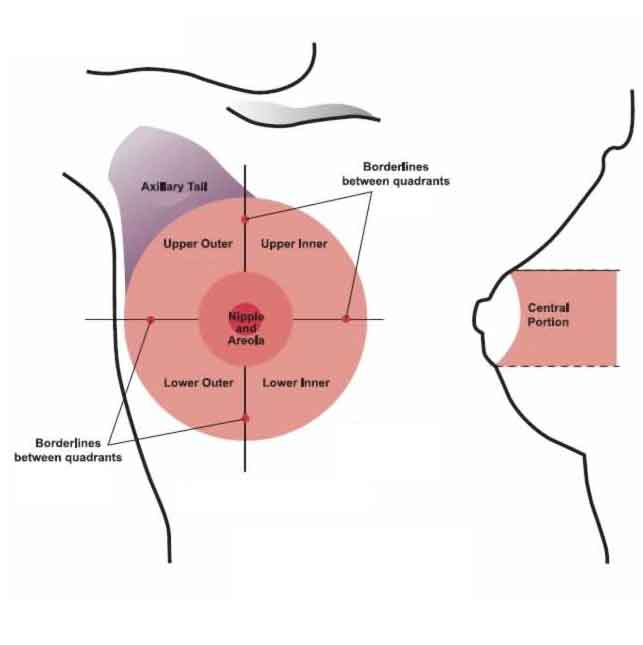
\includegraphics[width=0.5\textwidth]{breast_regions}
    \caption[Breast Regions]{Breast regions \protect\footnotemark}
    \label{fig:breast regions}
\end{center}
\end{figure}
\footnotetext{\url{https://www.pinterest.pt/pin/302304193710434456/}}

According to the study in \cite{Sohn2008}, 57\% of the breast cancer occurs in the upper-outer quadrant, 14\% in the upper-inner quadrant, 10\% in the lower-outer quadrant and 9\% in both the lower-inner quadrant 
and the nipple and areolar complex. The remaining 1\% occur in the axilliary tail.


With the increased concerned regarding cancer diseases, it has been made an effort to diagnose them as soon as possible. In the specific case of breast cancer, as shown in Figure~\ref{fig:breast_cancer_statistics}, 85\% of the patients who are diagnosed in early stages \footnote{ \url{http://www.cancerresearchuk.org/health-professional/cancer-statistics}} are granted a 90\% chance for the cancer be fully cured and provided with a survival rate greater than 88\%. All the diagnosed patients with stage I, II or part of stage III are considered early stages \footnote{\url{https://www.womenshealth.gov/publications/our-publications/fact-sheet/early-stage-breast-cancer.html}}. Early cancer diagnosing allows the patient not only to take less invasive treatments, but also have better aesthetic outcome at the end of treatment.

\begin{figure}[H]
\begin{center}
    \leavevmode
    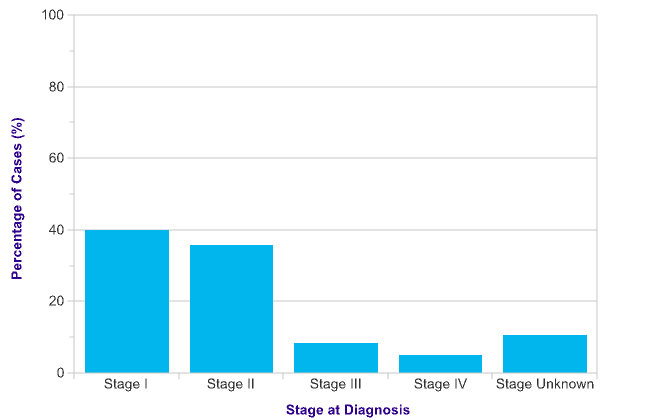
\includegraphics[width=0.85\textwidth]{inc_stage_breast_0}
    \caption[Breast cancer incidence by stage]{Breast cancer incidence by stage \protect\footnotemark}
    \label{fig:breast_cancer_statistics}
  \end{center}
\end{figure}
\footnotetext{\url{http://www.cancerresearchuk.org/health-professional/cancer-statistics/statistics-by-cancer-type/breast-cancer}}

Breast cancer is either considered as both invasive and non-invasive cancer as for spreading to surrounding tissues. The most common example of non-invasive breast cancer is known as Ductal Carcinoma in Situ (DCIS), in this case, the cancer is located on the place where the carcinoma occurred, growing through the milk ducts. If detected in early stages, this type of cancer can be easily cured with a great rate of success, otherwise it can evolve into an invasive breast cancer. On invasive breast cancer, the tumor spreads from the milk ducts and lobules to neighbor tissues. It can be classified in two different types of invasive breast cancer: Invasive Ductal Carcinoma, when the tumor has origin on the milk ducts; or Invasive Lobular Carcinoma, when the tumor has origin on the lobules.

The breast cancer can also be classified in different stages according with the size of the tumor and the affecting tissue.
The Stage 0, refers to the DCIS, with a few abnormal cells in lining of the ducts or small portions of the breast, and as a survival rate near 100\%;
The Stage 1, refers to breast cancer caused by carcinoma with less than 1 inch across (98\% survival rate); 
The Stage 2, refers to breast cancer caused by carcinoma with less than 2 inches across that can spread to some auxiliary lymph nodes  (88\% survival rate);
The Stage 3, refers to breast cancer caused by carcinoma larger than 2 inches across with an extensive spread to auxiliary or nearby lymph nodes. At this stage, some dimpling, inflammation or change of the color skin can be observed (52\% survival rate);
The Stage 4, refers to breast cancer caused by carcinoma spread from the breast to other regions and organs (16\% survival rate); \footnote{\url{http://johnstonhealth.org/2012/10/breast-cancer-awareness/}}

One of the most used and successful ways to diagnose breast cancer is thourgh MRI \footnote{\url{https://radiopaedia.org/articles/breast-mri}}; Mammograms also have an important role evaluating the risk for breast cancer growth, since the medical community has found breast tissue density an important factor for the growth of breast cancer \cite{Saidin2012}. Despite of the large number of breast density classifications, a fluently used is the Breast imaging-reporting and Data system (BIRADS) developed by the American College of Radiology (ACR) \cite{Saidin2012}.

The 4 categories defining the breast's density are enumerated below: \footnote{\url{https://radiopaedia.org/articles/breast-density}}
\begin{itemize}
\item \textbf{1} - fatty: breast is almost entirely fat;
\item \textbf{2} - scattered fibroglandular: breast has scattered areas of fibroglandular density;
\item \textbf{3} - heterogeneously dense: breast tissue is heterogeneously dense;
\item \textbf{4} - dense: breast tissue is extremely dense.
\end{itemize}

\section{Breast Cancer Treatment}\label{sec:treatment}

The goal of breast cancer treatment on early stages of the disease is to completely remove the cancer and preventing its recurrence. On later and more advanced stages of the cancer, it cannot be cured, so, the treatment techniques on this scenario focus on the attenuation of its effects and symptoms together with improving the QoL of the patient.

For years, the mastectomy has been the answer to treat breast cancer. Nowadays there are treatments with better results in terms of tumor removal and with a minor influence on the patients QoL, replacing the mastectomy by treatments such as BCS and oncoplastic treatments.

On the case of breast cancer on men, the mastectomy is always the recommended treatment option. However, for women, there are a lot of different treatment options that can vary between surgery to several therapies and a combination of them.

The treatments can be classified as local treatments or systemic treatments. The local treatments are applied on early cancer stages, treating tumors without affecting other parts of the body. When the cancer has already spread to surrounding tissues, systemic treatments are preferred in order to treat tumor cells on different areas of the patient's body. Some of the examples of local treatment are surgery and radiotherapy, while systemic treatments are composed by chemotherapy, hormone therapy or targeted therapy. This types of treatments may be combined to reach better results leading to two different types of therapy: neoadjuvant therapies and adjuvant therapies, that combine local and systemic treatments in order to treat a patient. The neoadjuvant therapy consists on applying systemic treatments before the surgery to reduce the carcinoma size. This allows to remove a smaller portion of the tumor during surgery and can be applied on cases that were considered inoperable due to the increased tumor size. The adjuvant therapy consists on complementary treatments applied after the surgery in order to eliminate cancer cells that may have spread previously to the surgery or eliminate cells not removed during the surgery \cite{De2016}.

As mentioned before, surgery is the most frequent option to treat breast cancer. However, it may be done for other reasons either than removing the tumor and the surrounding tissue, listed below:

\begin{itemize}
\item Perform biopsies on sentinel lymph nodes, in order to find if the cancer cells had spread to the axillary lymph nodes.
\item Breast reconstruction, to restore the breast shape after removing the tumor
\item Relieve symptoms of advanced breast cancer.
\end{itemize}

The most common types of surgery are Mastectomy and Breast Conserving Surgery, represented in Figure~\ref{fig:Breast Cancer Surgery}. Both are performed in order to remove the tumor and the surrounding tissue on the patient's breast.

\begin{figure}[H]
    \centering
    \subfloat[Mastectomy]{{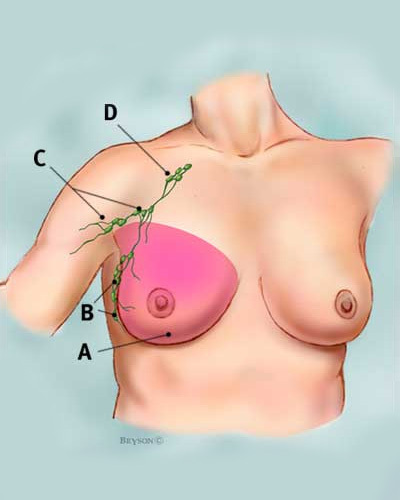
\includegraphics[width=5cm]{mastectomy} }}
    \qquad \qquad \qquad
    \subfloat[Breast Conserving Surgery]{{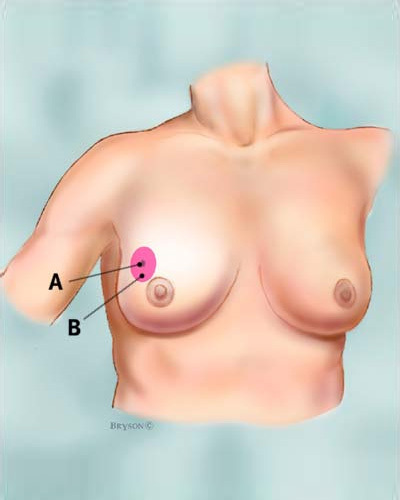
\includegraphics[width=5cm]{lumpectomy} }}
    \caption[Breast Cancer Surgery]{Breast Cancer Surgery \protect\footnotemark}
    \label{fig:Breast Cancer Surgery}
\end{figure}
\footnotetext{ \url{http://www.breastcancer.org/treatment/surgery}}

\begin{itemize}
\item \textbf{Mastectomy}

Even though the different approaches within the Mastectomy: radical mastectomy, modified radial mastectomy, simple mastectomy and skin-sparing mastectomy, all the above consists on the extraction of the entire breast tissues and some of the surrounding tissues. In the case of radical mastectomy, the pectoral muscle and all the axillary lymph nodes are also removed. Despite of the remotion of a great volume, the mastectomy do not remove tissues beyond the clavicle, the inframammary fold (above the rectus sheath), the midline of the sternum and the anterior border of the latissimus dorsi \cite{Witmer2004}. Less radical surgeries have been proved as effective as this. Nowadays, mastectomy is only performed for patients with large tumors that have spread into the pectoral muscle.

\item \textbf{Breast Conserving Surgery}

Breast Conserving Surgery (BCS), as known as partial mastectomy or lumpectomy, is a less extreme way to surgically remove the tumor. This procedure aims to remove the least possible amount of breast tissue, containing only the tumor and a small portion of the healthy tissue surrounding it. BCS is much less invasive than Mastectomy and with the same effectiveness and survival rates when radiotherapy is used as complementary treatment. Even though some women prefer the mastectomy, fearing the recurrence of the cancer, studies have proven that mastectomy do not provide any better result regarding the cancer treatment and recurrence than BCS, and the number of patients choosing this option as treatment has increased.
\end{itemize}

\section{Impact of Breast Cancer Treatment}

\subsection{Influence on the Aesthetic Outcome}

Several studies have been made in order to understand what parameters and how they influence the aesthetic outcome of BCS. These studies have evaluated parameters such as the age of the patient, her body mass index, the existence of palpable tumors, the location, volume and weight of the tumor, the axillary and breast incisions during surgery, among other factors.

It is also known that radiotherapy and chemotherapy have influence on the aesthetic result; however, all the studies regarding the adjuvant therapies influence are merely based on empirical experiences on patients.

According to \citet{Foersterling2014} previous studies have concluded that, generally, when the tumor is located on the inner quadrants of the breast, the treatment results in a poor aesthetic outcome. The location of the tumor on the nipple areolar complex leads to the most unfavorable aesthetic outcome. Unlike the location, the tumor weight has not been proved as predictive of a bad aesthetic outcome, in spite of tumors with less than 50g tend to lead to good aesthetic outcomes according with the aesthetic evaluation metrics presented in \cite{Joa2012}.

Concerning, the breast incision and besides of the inconsistent findings, some authors associate better aesthetic outcomes with radial and circular incisions, and worst outcomes with the periareolar one \cite{Foersterling2014}. Other studies point aspects like the result of mechanical forces such as gravity, breast tissue constitutive law distribution, inflammation due radiotherapy, the internal stress generated by the healing process and angiogenesis as factors on the breast shape after Breast Conserving techniques \cite{Vavourakis2016}. The aspect of the breast may change significantly during the healing process that can take as long as two years due to alteration regarding the tissue composition, stiffness and volume.

\subsection{Quality of Life}

Changes of the breast's size or shape or even the loss of it have a significant impact on the psychological and social life of a patient. The loss of breast as a symbol of femininity has may lead to a decrease of the patient's self-esteem, negative body image, social isolation and communication and relationship problems. The psychosocial stress and the physical burden may result in a reduction of the patient's opportunities in life and increase their social rejection. Common symptoms of the breast cancer treatment visible on a wide number of patients are anxiety, depression, fatigue, pain, difficult in concentration, sexuality concerns and self-blame \cite{Al-Azri2014}. Despite of the sparsity of studies regarding the influence of breast treatment surgeries on women's body image and sexuality, the most recent ones consider BCS result on a best preservation of the woman's body image and more comfort about their sexuality \cite{Rowland2000}.

\section{Summary}

Given the importance of the visualization of a treatment outcome on a breast cancer treatment and the impact it has on the QoL of the patient, the ability of predicting the aesthetic outcome of a surgery is a valuable aspect.

Currently, this is shown with 2D drawings and pictures of similar cases, and in some cases with generic 3D models. A patient-specific prediction will allow to minimize the doctor-patient misunderstandings, to find the optimal treatment, to decrease the fear the patients stood against surgery and to select the most desired outcome of the surgery. In order to achieve this, it is important to be able to manipulate a 3D breast model, and define the transformations that each treatment may led on the patient's breast. As outcome, the patient may be able to see own breast deformed in a real time system.

The next chapter describes the models that are being used so far and how a breast model may be represented as well as some existing simulations of the breast surgery.
